\chapter{Acquiring Annotation from Human Experts}
\label{ch3}

This chapter is based on the following publications:
\begin{itemize}
    \item Zhou, Z., Shin, J., Zhang, L., Gurudu, S., Gotway, M., \& Liang, J. (2017). Fine-tuning convolutional neural networks for biomedical image analysis: actively and incrementally. In \textit{Proceedings of the IEEE conference on computer vision and pattern recognition} (pp. 7340-7351).
    \item Zhou, Z., Shin, J., Feng, R., Hurst, R. T., Kendall, C. B., \& Liang, J. (2019). Integrating active learning and transfer learning for carotid intima-media thickness video interpretation. \textit{Journal of digital imaging}, 32(2), 290-299.
    \item Zhou, Z., Shin, J. Y., Gurudu, S. R., Gotway, M. B., \& Liang, J. (2021). Active, Continual Fine Tuning of Convolutional Neural Networks for Reducing Annotation Efforts. \textit{Medical Image Analysis}, 101997.
\end{itemize}

% \section*{CRediT authorship contribution statement}

% I would like to thank all of the authors for their contributions and hard works. Jae Y. Shin: software, investigation, visualization. Suryakanth R. Gurudu: resources, data curation. Michael B. Gotway: resources, data curation, funding acquisition. Jianming Liang: conceptualization, methodology, formal analysis, investigation, resources, writing, supervision, project administration, funding acquisition. 

\newpage


\section{Background \& Motivation}
\label{ch3:backgroun_motivation}

Convolutional neural networks (CNNs)~\citep{lecun2015deep} have ushered in a revolution in computer vision owing to the use of large annotated datasets, such as \textsc{ImageNet}~\citep{deng2009imagenet} and \textsc{Places}~\citep{zhou2017places}. As evidenced by two recent books~\citep{shen2019medical,zhou2019handbook} and numerous compelling techniques for different imaging tasks~\citep{moen2019deep,yamamoto2019automated,ravizza2019predicting,esteva2019guide,huang2020penet,isensee2021nnu}, there is widespread and intense interest in applying CNNs to medical image analysis, but the adoption of CNNs in medical imaging is hampered by the lack of such large annotated datasets. Annotating medical images is not only tedious and time consuming, but it also requires costly, specialty-oriented knowledge and skills, which are not readily accessible. Therefore, we seek to answer this critical question: {\em How to dramatically reduce the cost of annotation when applying CNNs to medical imaging}?
In doing so, we have developed a novel method called ACFT (active, continual fine-tuning) to naturally integrate active learning and transfer learning into a single framework. Our ACFT method starts directly with a pre-trained CNN to seek ``salient'' samples from the unannotated pool for annotation, and the (fine-tuned) CNN is continually fine-tuned using newly annotated samples combined with all misclassified samples. We have evaluated our method in three different applications, including colonoscopy frame classification, polyp detection, and pulmonary embolism (PE) detection, demonstrating that the cost of annotation can be reduced by at least half.

This performance is attributable to a simple yet powerful observation: to boost the performance of CNNs in medical imaging, multiple patches are usually generated automatically for each sample through data augmentation; these patches generated from the same sample share the same label, and are naturally expected to have similar predictions by the current CNN before they are expanded into the training dataset. As a result, their {\em entropy}~\citep{shannon1948mathematical} and {\em diversity}~\citep{kukar2003transductive} provide a useful indicator of the ``power'' of a sample for elevating the performance of the current CNN. However, automatic data augmentation inevitably generates ``hard'' samples, injecting noisy labels. Therefore, to significantly enhance the robustness of active selection, we compute entropy and diversity from only a portion of the patches according to the majority predictions detailed in Sec.~\ref{ch3:approach_property:handling_noisy_labels_majority_selection}) by the current CNN. 
Furthermore, to strike a balance between exploration and exploitation, we incorporate randomness in our active selection as detailed in Sec.~\ref{ch3:approach_property:injecting_randomization_active_selection}; and to prevent catastrophic forgetting, we combine newly selected samples with misclassified samples as described in Sec.~\ref{ch3:experiment_result:comparing_four_active_learning_strategies}.

To our knowledge, our proposed method is among the first to integrate active learning into fine-tuning CNNs in a continual fashion to make CNNs more amenable to medical image analysis, particularly with the intention of decreasing the efforts of annotation dramatically. Compared with conventional active learning, our work makes the following contributions:

\begin{enumerate}
    \item We devise novel active learning criteria, which select the most informative samples by considering both prediction certainty and consistency.
    \item We develop various continual fine-tuning strategies, which efficiently utilize the newly annotated and misclassified samples.
\end{enumerate}

%%%%%%%%%%%%%%%%%%%%%%%%%%%%%%%%%%%%%%%%%%%%
% \begin{landscape}
% \thispagestyle{empty}

\begin{sidewaysfigure}
\begin{center}
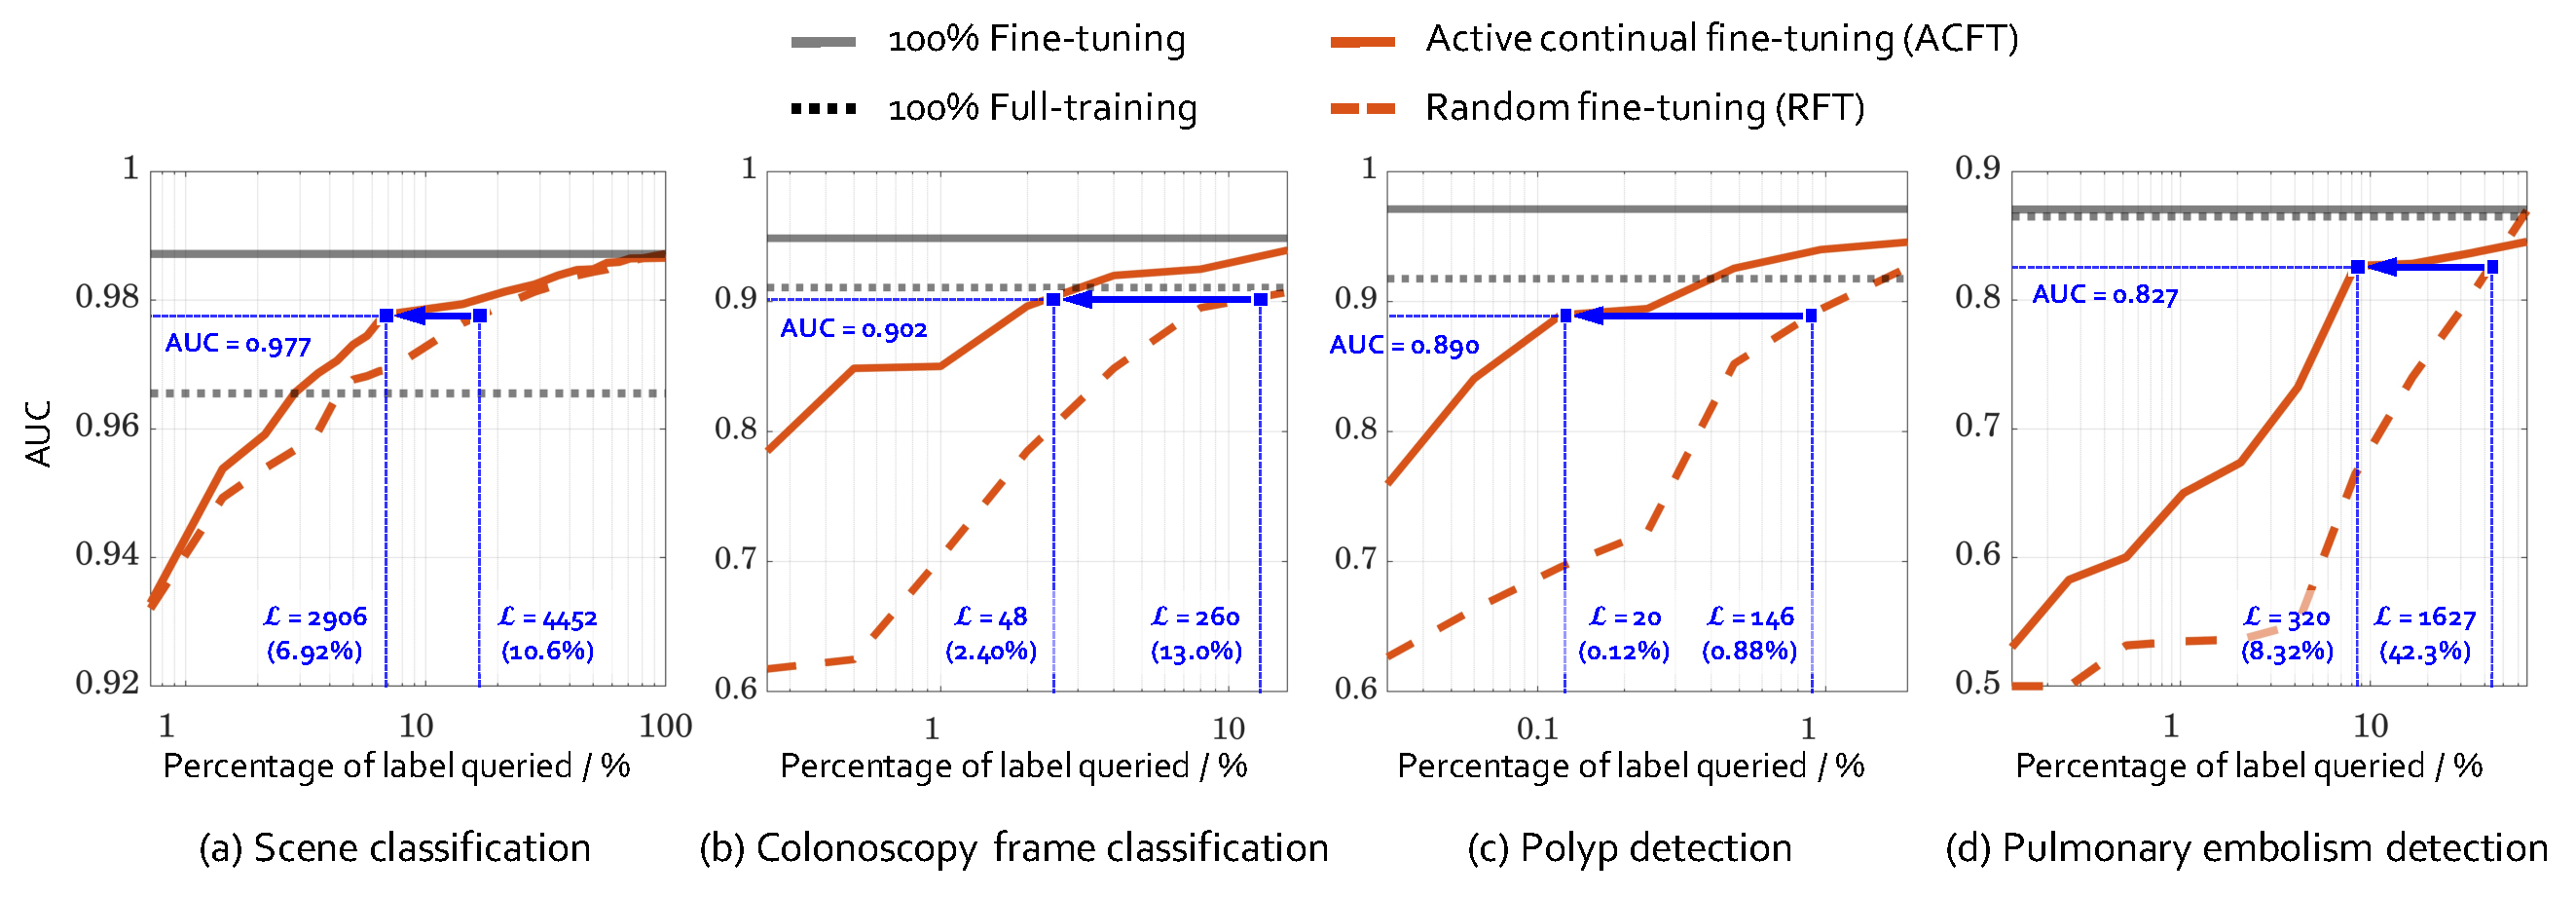
\includegraphics[width=0.95\columnwidth]{Figures/CH3/fig_result_highlights.pdf}
\end{center}
\caption[Active Continual Fine-tuning Reduces over 80\% Annotation Cost]{
ACFT aims to minimize the number of samples for experts to label by iteratively recommending the most informative and representative samples. For scene classification (a), by actively selecting 2,906 images (6.92\% of the entire dataset), ACFT can offer equivalent performance to the use of 4,452 images through random selection, thus saving 34.7\% annotation cost relative to random fine-tuning. Furthermore, with 1,176 actively-selected images (2.80\% of the whole dataset), ACFT can achieve performance equivalent to full training using 42,000 images, thereby saving 97.2\% annotation cost (relative to full training). 
In (b)---(d), we highlight the major results that compared with RFT, our ACFT can reduce the cost of annotation by 81.5\% for colonoscopy frame classification, 86.3\% for polyp detection, and 80.3\% for pulmonary embolism detection. 
% Following the standard active learning experimental setup, both ACFT and RFT select samples from the remaining training dataset; they will eventually use the same whole training dataset, naturally yielding similar performance at the end. However, the goal of active learning is to find such sweet spots where a learner can achieve an acceptable performance using the least number of labeled samples.
}
\label{ch3:fig:overall_result}
\end{sidewaysfigure}

% \fillandplacepagenumber
% \end{landscape}
%%%%%%%%%%%%%%%%%%%%%%%%%%%%%%%%%%%%%%%%%%%%







%%%%%%%%%%%%%%%%%%%%%%%%%%%%%%%%%%%%%%%%%%%%
\begin{algorithm}[t]
% \singlespace
\footnotesize
\caption{ACFT -- Active, Continual Fine-Tuning}
\label{ch3:alg:ACFT}
    \KwIn{\\
    \ \ \ $\mathcal{U}=\{\mathcal{C}_i\},$ $i\in [1,n]$ \{unlabeled pool $\mathcal{U}$\ contains $n$ candidates\}\\
    \ \ \ $\mathcal{C}_i=\{x_i^j\}$, $j\in [1,m]$ \{each $\mathcal{C}_i$ contains $m$ patches\}\\
    \ \ \ $M_0$: pre-trained CNN;
    \ $\alpha$: majority ratio;
    \ $b$: batch size;
    \ $\mathcal{Y}$: category set
    }
    \KwOut{\\
    \ \ \ $\mathcal{L}$: labeled candidates;
    \ $M_t$: fine-tuned CNN model at Step $t$
    }
    $\mathcal{L} \leftarrow \varnothing$;
    \ $t\leftarrow 1$\\
    \Repeat{ classification performance in a validation set plateaus}{

    \For{ each $\mathcal{C}_i \in \mathcal{U}$ }
    {
        $P_i \leftarrow M_{t-1}(\mathcal{C}_i)$ \{outputs of $M_{t-1}$ given $\forall x \in \mathcal{C}_i$\}\\
        $\mathcal{C}'_i \leftarrow \mathcal{C}_i$ descending sort on the predicted dominant class $\hat{\textbf{y}}_i$ by Eq.~\ref{eq:dominate_class} \\
        $\mathcal{C}^{\alpha}_i \leftarrow$ top $\alpha\times 100\%$ of the patches of the sorted list $\mathcal{C}'_i$ \\
        Compute $\textbf{\em a}_i$ for $\mathcal{C}^{\alpha}_i$ by Eq.~\protect\ref{eq:R}, \ie $\textbf{\em a}_i =\lambda_1 \textbf{\em e}_i+\lambda_2 \textbf{\em d}_i\quad$ \\
    }
    Sort $\mathcal{U}$ according to $\textbf{\em a}$ in descending order\\
    Compute sampling probability $\textbf{\em a}^{s}$ using sorted list $\textbf{\em a}'$ by Eq.~\ref{eq:randomness} \\
    Associate labels for $b$ candidates with sampling probabilities: $\mathcal{Q}\leftarrow Q(\textbf{\em a}^{s},b)$ \\
    $P \leftarrow M_{t-1}(\mathcal{L})$ \{outputs of $M_{t-1}$ given $\forall x \in \mathcal{L}$\} \\
    Select misclassified candidates from $\mathcal{L}$ based on their annotation: $\mathcal{H} \leftarrow J(P, \mathcal{L})$ \\
    Fine-tune $M_{t-1}$ with $\mathcal{H}\bigcup\mathcal{Q}$: $M_t \leftarrow F(\mathcal{H}\bigcup\mathcal{Q},M_{t-1})$  \\
    $\mathcal{L} \leftarrow  \mathcal{L}\bigcup \mathcal{Q};  \quad \mathcal{U} \leftarrow \mathcal{U} \setminus \mathcal{Q};  \quad t\leftarrow t+1$ \\
    }
\end{algorithm}
%%%%%%%%%%%%%%%%%%%%%%%%%%%%%%%%%%%%%%%%%%%%



\section{Approach \& Property}
\label{ch3:approach_property}



Active, continual fine-tuning (ACFT) was conceived in the context of computer-aided diagnosis (CAD) applied to medical imaging. A CAD system typically employs a candidate generator, which can quickly produce a set of candidates,  among which some are true positives and others are false positives. To train a classifier, each of the candidates must be labeled. In this work, an object to be labeled is considered as a ``candidate'' in general. We assume that each candidate takes one of $|\mathcal{Y}|$ possible labels.  To boost CNN performance for CAD systems, multiple patches are usually generated automatically for each candidate through data augmentation; those patches that are generated from the same candidate inherit the candidate's label. In other words, all labels are acquired at the candidate level. Mathematically, given a set of candidates, $\mathcal{U}=\{\mathcal{C}_1, \mathcal{C}_2, ..., \mathcal{C}_n\}$, where $n$ is the number of candidates, and each candidate $\mathcal{C}_i =\{x^{1}_i,x^{2}_i,...,x^{m}_i\}$ is associated with $m$ patches, our ACFT  algorithm iteratively selects a set of candidates for labeling as illustrated in~Alg.~\ref{ch3:alg:ACFT}.



\subsection{Selecting Based on Certainty and Consistency}
\label{ch3:approach_property:selection_certainty_consistency}

In active learning, the key is to develop criteria for determining ``worthiness'' of labeling a candidate. Our criteria for candidate ``worthiness'' are based on a simple, yet powerful, observation: all patches augmented from the same candidate share the same label; therefore, they are expected to have similar predictions by the current CNN. As a result, their {\em entropy} and {\em diversity} provide a useful indicator of the ``power'' of a candidate for elevating the performance of the current CNN. Intuitively, entropy captures classification certainty---a higher uncertainty value denotes a greater degree of information, whereas diversity indicates prediction consistency among the candidate patches---a higher diversity value denotes a greater degree of prediction inconsistency. Formally, assuming that each candidate takes one of $|\mathcal{Y}|$ possible labels, we define the entropy and diversity of $\mathcal{C}_i$ as

\begin{equation}
\label{eq:active_criteria}
\begin{split}
&\textbf{\em e}_i = -\frac{1}{m}\sum_{k=1}^{|\mathcal{Y}|}{\sum_{j=1}^{m}{P_i^{j,k}\log{P_i^{j,k}}}}, \\
&\textbf{\em d}_i = \sum_{k=1}^{|\mathcal{Y}|}{\sum_{j=1}^m{\sum_{l=j}^m{(P_i^{j,k}-P_i^{l,k})\log{\frac{P_i^{j,k}}{P_i^{l,k}}}}}}
\end{split}
\end{equation}
Combining entropy and diversity yields
\begin{equation}
\label{eq:R}
\textbf{\em a}_i =\lambda_1 \textbf{\em e}_i+\lambda_2 \textbf{\em d}_i
\end{equation}
where $\lambda_1$ and $\lambda_2$ are trade-offs between entropy and diversity. We use two parameters for convenience,  to easily turn on/off entropy or diversity during experiments.




\subsection{Handling Noisy Labels via Majority Selection}
\label{ch3:approach_property:handling_noisy_labels_majority_selection}

Automatic data augmentation is essential for boosting CNN performance, but it inevitably generates ``hard'' samples for some candidates, as shown in \figurename~\ref{ap1:fig:dataset_annotation}(c), injecting noisy labels. Therefore, to significantly enhance the robustness of our method, we compute entropy and diversity by selecting only a portion of the patches of each candidate according to the predictions by the current CNN.

Specifically, for each candidate $\mathcal{C}_i$ we first determine its dominant category, which is defined by the category with the highest confidence in the mean prediction. That is,
\begin{equation}
\label{eq:dominate_class}
\hat{\textbf{y}}_i =  \argmax_{y \in \mathcal{Y}} \frac{1}{m}\sum_{j=1}^{m}P^{j,y}_i
\end{equation}
where $P^{j,y}_i$ is the output of each patch $j$ from the current CNN given $\forall x \in \mathcal{C}_i$ on label $y$. After sorting $P_i$ according to dominant category $\hat{\textbf{y}}_i$, we apply Eq.~\ref{eq:R} to top $\alpha\times$100\% of the patches to construct the score matrix $\textbf{\em a}_i$ of size $\alpha m \times \alpha m$ for each candidate $\mathcal{C}_i$ in $\mathcal{U}$. Our proposed majority selection method automatically excludes those patches with noisy labels owning to their high consistency in the majority of predictions.

%%%%%%%%%%%%%%%%%%%%%%%%%%%%%%%%%%%%%%%%%%%%
% \begin{landscape}
% \thispagestyle{empty}

\begin{sidewaysfigure}
\begin{center}
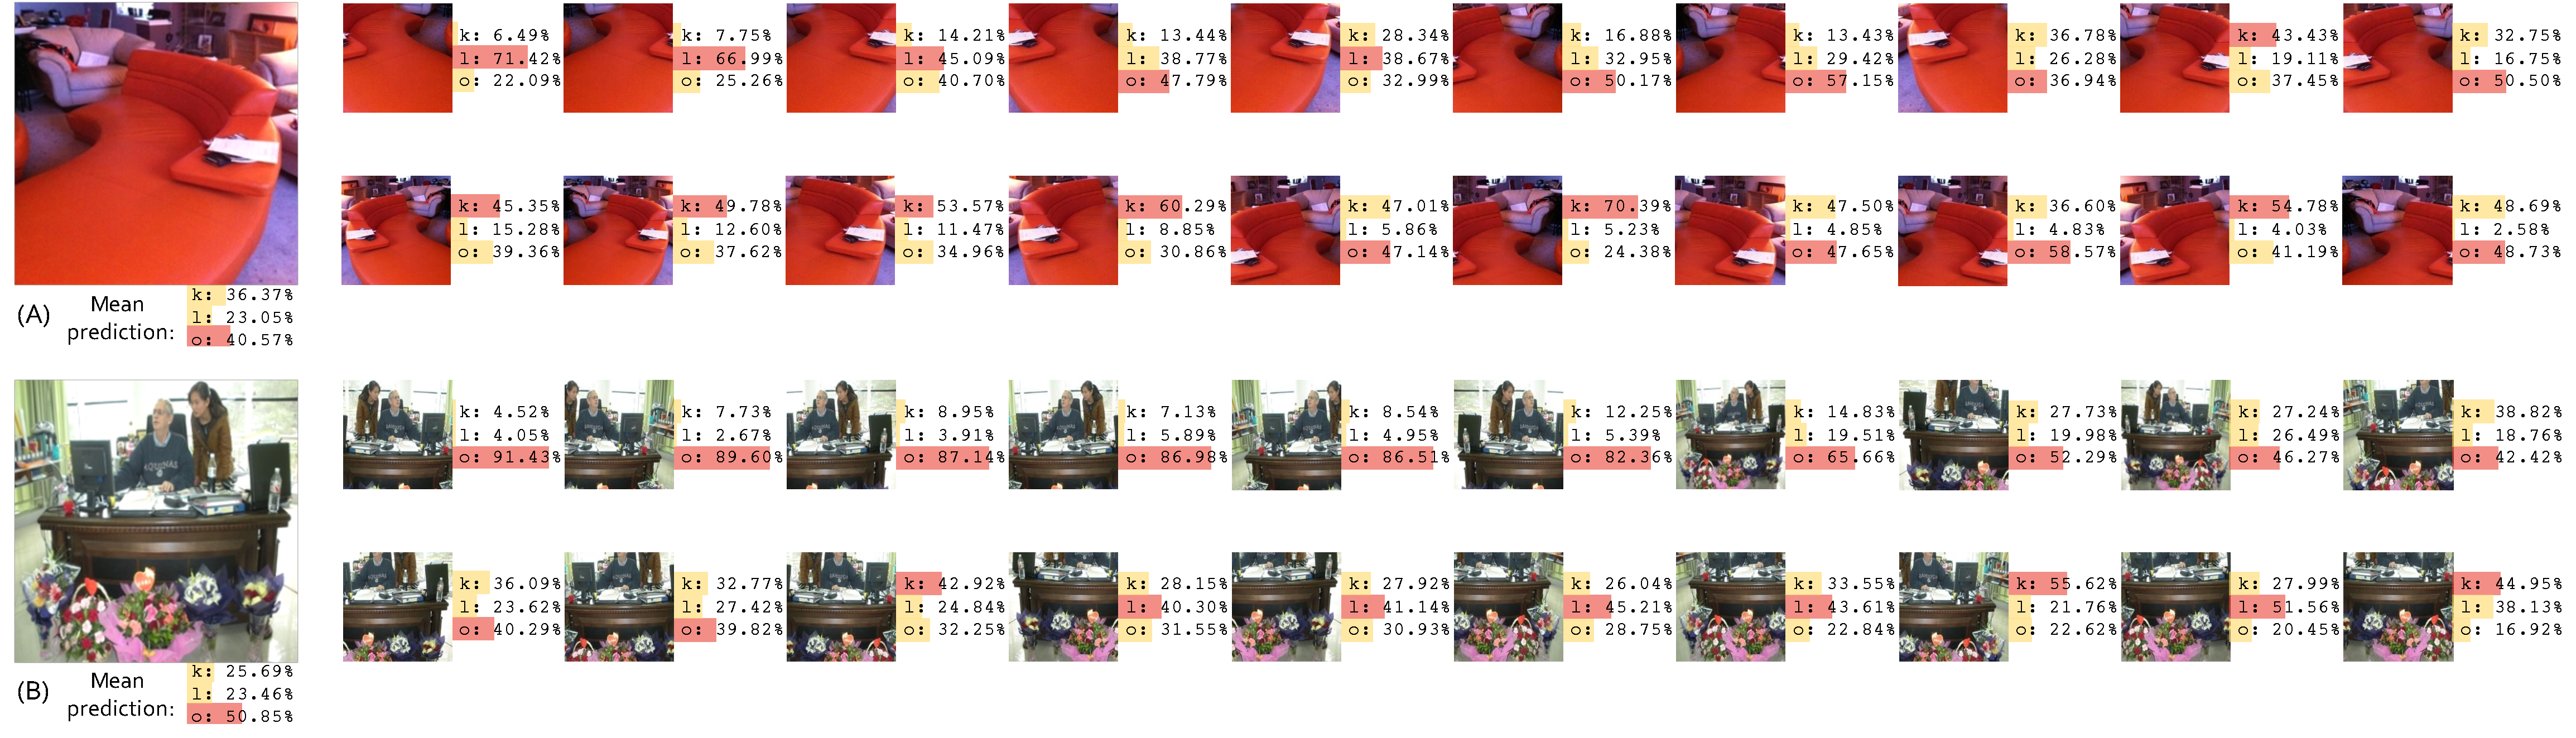
\includegraphics[width=1.0\columnwidth]{Figures/CH3/fig_data_augumentation.pdf}
\end{center}
\caption[The Significance of Majority Selection]{
% Automatic data augmentation inevitably generates noisy patches, and there is no need to classify all patches confidently. 
% Therefore, we propose majority selection, which computes active selection criteria on only the top 25\% of the patches with the highest confidences on the dominant predicted category.
To demonstrate the necessity of majority selection, we illustrate two images (A and B) and their augmented patches, arranged according to the dominant category predicted by the CNN. 
Based on \textsc{Places-3}, Image A is labeled as {\em living room}, and its augmented patches are mostly incorrectly classified by the current CNN; therefore, including it in the training set is of great value. On the contrary, Image B is labeled as {\em office}, and the current CNN classifies most of its augmented patches as {\em office} with high confidence; labeling it would be of limited utility. 
Without majority selection, the criteria would mislead the selection, as it indicates that Image B is more diverse than Image A (297.52 vs. 262.39) while sharing similar entropy (17.33 vs. 18.50). With majority selection, the criteria show that Image A is considerably more uncertain and diverse than Image B, measured by either entropy (4.59 vs. 2.17) or diversity (9.32 vs. 0.35), and as expected, more worthy of labeling. From this active selection analysis, we remark that the majority selection is a critical component in our ACFT.
}
\label{ch3:fig:places_examples}
\end{sidewaysfigure}

% \fillandplacepagenumber
% \end{landscape}
%%%%%%%%%%%%%%%%%%%%%%%%%%%%%%%%%%%%%%%%%%%%



\subsection{Injecting Randomization into Active Selection}
\label{ch3:approach_property:injecting_randomization_active_selection}

As discussed in~\citet{borisov2010active} and~\citet{zhou2017fine}, simple random selection may outperform active selection at the beginning, because the active selection method depends on the current model selecting examples for labeling. As a result, a poor selection made at an early stage may adversely affect the quality of subsequent selections, whereas the random selection approach is less frequently locked into a poor hypothesis. In other words, the active selection method concentrates on exploiting the knowledge gained from the labels already acquired to further explore the decision boundary, whereas the random selection approach concentrates solely on exploration, and is thereby able to locate areas of the feature space where the classifier performs poorly. Therefore, an effective active learning strategy must strike a balance between exploration and exploitation.
Towards this end, we inject randomization into our method by selecting actively according to the sampling probability $\textbf{\em a}^{s}_i$.

\begin{equation}
\label{eq:randomness}
\begin{split}
\textbf{\em a}'_i=(\textbf{\em a}'_i-\textbf{\em a}'_{\omega b})/(\textbf{\em a}'_1-\textbf{\em a}'_{\omega b}), \\
 \textbf{\em a}^{s}_i=\textbf{\em a}'_i/\sum_i{\textbf{\em a}'_i},\quad \forall i \in [1,\omega b]
\end{split}
\end{equation}
where $\textbf{\em a}'_i$ is sorted $\textbf{\em a}_i$ according to its value in descending order, and $\omega$ is named random extension.
Suppose $b$ number of candidates are required for annotation. Instead of selecting top $b$ candidates, we extend the candidate selection pool to $\omega b$. Then we select candidates from this pool with their sampling probabilities $\textbf{\em a}^{s}_i$ to inject randomization.


\subsection{Five Unique Properties}
\label{ch3:approach_property:several_unique_properties}


\begin{enumerate}[noitemsep]

    \item \textit{ACFT integrates entropy and diversity.} Our algorithm actively selects the most uncertain and informative candidates by naturally exploiting expected consistency among the patches within each candidate, reducing the number of redundancy and outliers. 
    
    \item \textit{ACFT overcomes noisy labels associated with augmentation.} Our algorithm computes selection criteria locally on a small number of patches within each candidate, saving considerable computation cost for diversity metric.
    
    \item \textit{ACFT tackles cold start problem by injecting randomness.} Our algorithm balances exploration and exploitation by incorporating randomness into active selection, demonstrating the superior performance even at the beginning of active learning procedure.
    
    \item \textit{ACFT balances training samples among classes.} Our algorithm seeks the most critical candidates to be annotated for the current model, ensuring a comparable number of candidates selected from minority classes and preventing the model from being skewed towards majority classes.
    
    \item \textit{ACFT is generic and applicable to many imaging tasks.} Our algorithm was initially developed for the purpose of medical imaging, but it also demonstrates over 30\% annotation reduction for the scene classification task in natural imaging as well. We illustrate the ideas behind ACFT with the \textsc{Places-3} dataset~\citep{zhou2017places}, where no candidate generator is needed, as each image may be directly regarded as a candidate. 

\end{enumerate}



\section{Experiment \& Result}
\label{ch3:experiment_result}

In this section, \figurename~\ref{ch3:fig:overall_result} begins with an overall performance between our active continual fine-tuning (ACFT) and random fine-tuning (RFT), revealing the amount of annotation effort that has been reduced in each application. \figurename~\ref{ch3:fig:selection_approaches_comparison_alexnet} and \figurename~\ref{ch3:fig:selection_approaches_comparison_googlenet} compare eight different active selecting criteria, demonstrating that majority selection and randomness are critical in finding the most representative samples to elevate the current CNN's performance.
\figurename~\ref{ch3:fig:predicted_distribution} further presents the observed distribution of each active selecting criteria, qualitatively confirming the rationale of our devised candidate selecting approaches.
\tableautorefname~\ref{ch3:tab:main_results} finally compares four different active learning strategies, suggesting that continual fine-tuning using newly annotated candidates enlarged by those misclassified candidates significantly saves computational resources while maintaining the compelling performance in all three medical applications.

%%%%%%%%%%%%%%%%%%%%%%%%%%%%%%%%%%%%%%%%%%%%
\begin{table}[t]
\begin{center}
\begin{threeparttable}
\footnotesize
\caption[Abbreviation and Definition of Learning Strategies]{
Active learning strategy definition. We have codified different learning strategies covering the makeup of training samples and the initial model weights of fine-tuning.}
\label{ch3:tab:terminology}
    \begin{tabular}{p{0.15\textwidth}p{0.8\textwidth}}
    \hline
    \textbf{Code} & \textbf{Description of learning strategy} \\
    \hline
    RFT$_{(LQ)}$ & Fine-tuning from $M_{0}$ using $\mathcal{L}$ and randomly selected $\mathcal{Q}$ \\
    AFT$_{(LQ)}$ & Fine-tuning from $M_0$ using $\mathcal{L}$ and actively selected $\mathcal{Q}$ \\
    ACFT$_{(Q)}$ & Continual fine-tuning from $M_{t-1}$ using actively selected $\mathcal{Q}$ only \\
    ACFT$_{(LQ)}$ & Continual fine-tuning from $M_{t-1}$ using $\mathcal{L}$ and actively selected $\mathcal{Q}$ \\
    ACFT$_{(HQ)}$ & Continual fine-tuning from $M_{t-1}$ using $\mathcal{H}$ and actively selected $\mathcal{Q}$ \\
    \hline
    \end{tabular}
    \begin{tablenotes}
        \footnotesize
        \item[1] $\mathcal{L}$: Labeled candidates.
        \item[2] $\mathcal{Q}$: Newly annotated candidates.
        \item[3] $\mathcal{H}$: Misclassified candidates.
        \item[4] $M_0$: Pre-trained CNNs from large scale dataset (like \textsc{ImageNet}).
        \item[5] $M_{t-1}$: Pre-trained CNNs from last active selecting iteration.
    \end{tablenotes}
\end{threeparttable}
\end{center}
\end{table}
%%%%%%%%%%%%%%%%%%%%%%%%%%%%%%%%%%%%%%%%%%%%


%%%%%%%%%%%%%%%%%%%%%%%%%%%%%%%%%%%%%%%%%%%%
\begin{table}[t]
\caption[Analysis on Active Selection Pattern]{
Active selection patterns analysis. We illustrate the relationships among seven prediction patterns and four active selection criteria, assuming that a candidate $\mathcal{C}_i$ has 11 augmented patches, and their probabilities $P_i$ are predicted by the current CNN, presented in the second column. With majority selection, the entropy and diversity are calculated based on the top 25\% (3 patches in this illustration) highest confidences on the dominant predicted category. The first choice of each method (column) is \textbf{bolded} and the second choice is \underline{underlined}.
}
\label{ch3:tab:predict_pattern}
\begin{center}
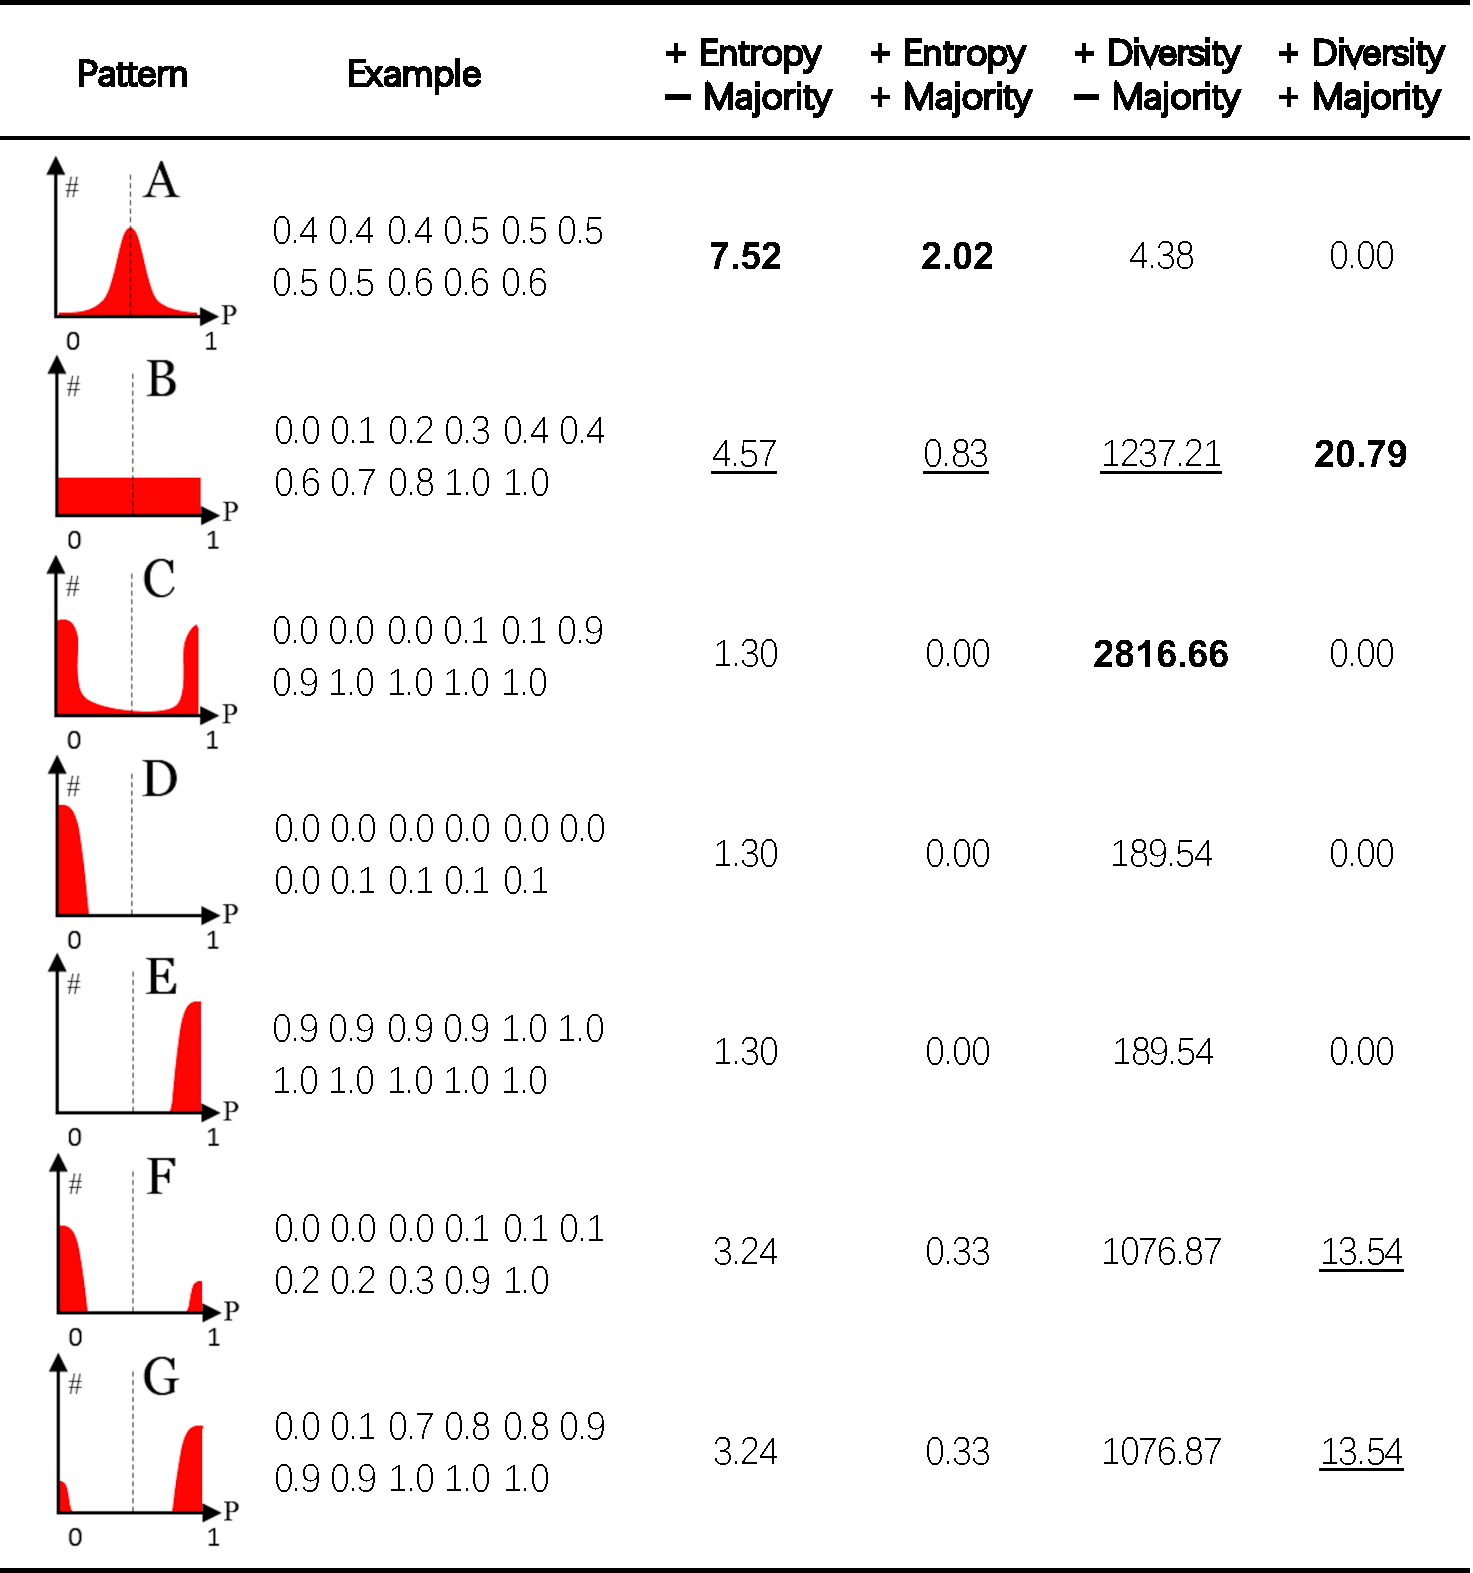
\includegraphics[width=0.7\linewidth]{Figures/CH3/fig_hypothsis_pattern.pdf}\\
\end{center}
\end{table}
%%%%%%%%%%%%%%%%%%%%%%%%%%%%%%%%%%%%%%%%%%%%

\subsection{Benchmarking Active, Continual Fine-Tuning}
\label{sch2:experiment_result:benchmarking_active_continual_finetuning}


\citet{tajbakhsh2016convolutional} reported the state-of-the-art performance of fine-tuning and learning from scratch using entire datasets, which are used to establish baseline performance for comparison. These authors also investigated the performance of (partial) fine-tuning using a sequence of partial training datasets, but our dataset partitions are different from theirs. Therefore, for a fair comparison with their approach, we introduce RFT, which fine-tunes the original model $M_0$  from the beginning, using all available labeled samples $\mathcal{L}\bigcup\mathcal{Q}$, where $\mathcal{Q}$ is randomly selected at each step. 

We summarized several active learning strategies in \tableautorefname~\ref{ch3:tab:terminology}. Studying different active learning strategies is important because active learning procedure can be very computationally inefficient in practice, in terms of label reuse and model reuse. We present two strategies that aim at overcoming the above limitations. First, we propose to combine newly annotated data with the labeled data that is misclassified by the current CNN. Second, we propose continual fine-tuning to speed up model training and, in turn, encourage data reuse.
ACFT$_{(HQ)}$ denotes the optimized learning strategy, which continually fine-tunes the current model $M_{t-1}$ using newly annotated candidates enlarged by those misclassified candidates; that is, $\mathcal{Q}\bigcup\mathcal{H}$. 
Compared with other learning strategy baselines~\citep{tajbakhsh2016convolutional, zhou2017fine,zhou2019integrating} as codified in \tableautorefname~\ref{ch3:tab:terminology}, ACFT$_{(HQ)}$ saves training time through faster convergence compared with repeatedly fine-tuning the original pre-trained CNN, and boosts performance by eliminating easy samples, focusing on hard samples, and preventing catastrophic forgetting. In all three applications, our ACFT begins with an empty training dataset and directly uses pre-trained models (AlexNet and GoogLeNet) on ImageNet.


\subsection{Assessing Eight Active Selecting Criteria}
\label{ch3:experiment_result:assessing_eight_active_selecting_criteria}

We meticulously monitored the active selection process and examined the selected candidates. For example, we include the top ten candidates selected by the four ACFT methods at Step 3 in colonoscopy frame classification in \figurename~\ref{ch3:fig:predicted_distribution}. From this process, we have observed the following:
\begin{itemize}
\item Patterns A and B are dominant in the earlier stages of ACFT as the CNN has not been fine-tuned properly to the target domain;
\item Patterns C, D and E are dominant in the later stages of ACFT as the CNN has been largely fine-tuned on the target dataset;
\item Majority selection is effective for excluding Patterns C, D, and E, whereas entropy only (without the majority selection) can handle Patterns C, D, and E reasonably well;
\item Patterns B, F, and G generally make good contributions to elevating the current CNN's performance;
\item Entropy and entropy+majority favor Pattern A due to its higher degree of uncertainty, and;
\item Diversity+majority prefers Pattern B whereas diversity prefers Pattern C. This is why diversity may cause sudden disturbances in the CNN's performance and why diversity+majority is generally preferred.

\end{itemize}

%%%%%%%%%%%%%%%%%%%%%%%%%%%%%%%%%%%%%%%%%%%%
% \begin{landscape}
% \thispagestyle{empty}

% \begin{figure}[t]
\begin{sidewaysfigure}
\begin{center}
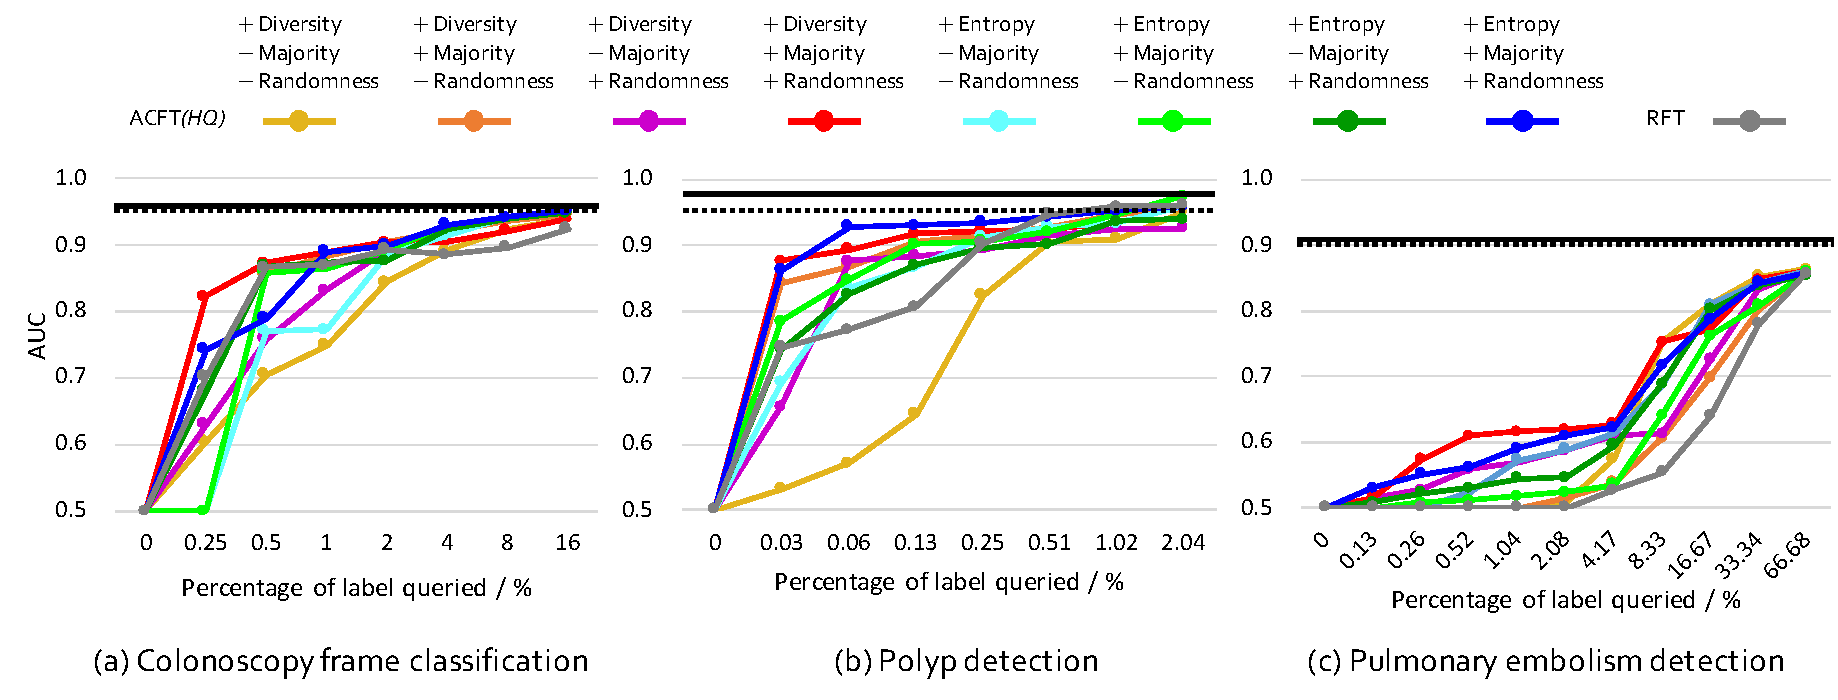
\includegraphics[width=1.0\columnwidth]{Figures/CH3/fig_selection_approaches_comparison_alexnet.pdf}
\end{center}
\caption[Assessment of Eight Active Selecting Criteria (AlexNet)]{
Comparing eight active selection approaches with random selection on AlexNet~\citep{krizhevsky2012imagenet} for our three distinct medical applications, including (a) colonoscopy frame classification, (b) polyp detection, and (c) pulmonary embolism detection, demonstrates consistent patterns with AlexNet. The solid black line denotes the current state-of-the-art performance of fine-tuning using full training data and the dashed black line denotes the performance of training from scratch using full training data.}
\label{ch3:fig:selection_approaches_comparison_alexnet}
\end{sidewaysfigure}
% \end{figure}

% \fillandplacepagenumber
% \end{landscape}
%%%%%%%%%%%%%%%%%%%%%%%%%%%%%%%%%%%%%%%%%%%%

%%%%%%%%%%%%%%%%%%%%%%%%%%%%%%%%%%%%%%%%%%%%
% \begin{landscape}
% \thispagestyle{empty}

\begin{sidewaysfigure}
\begin{center}
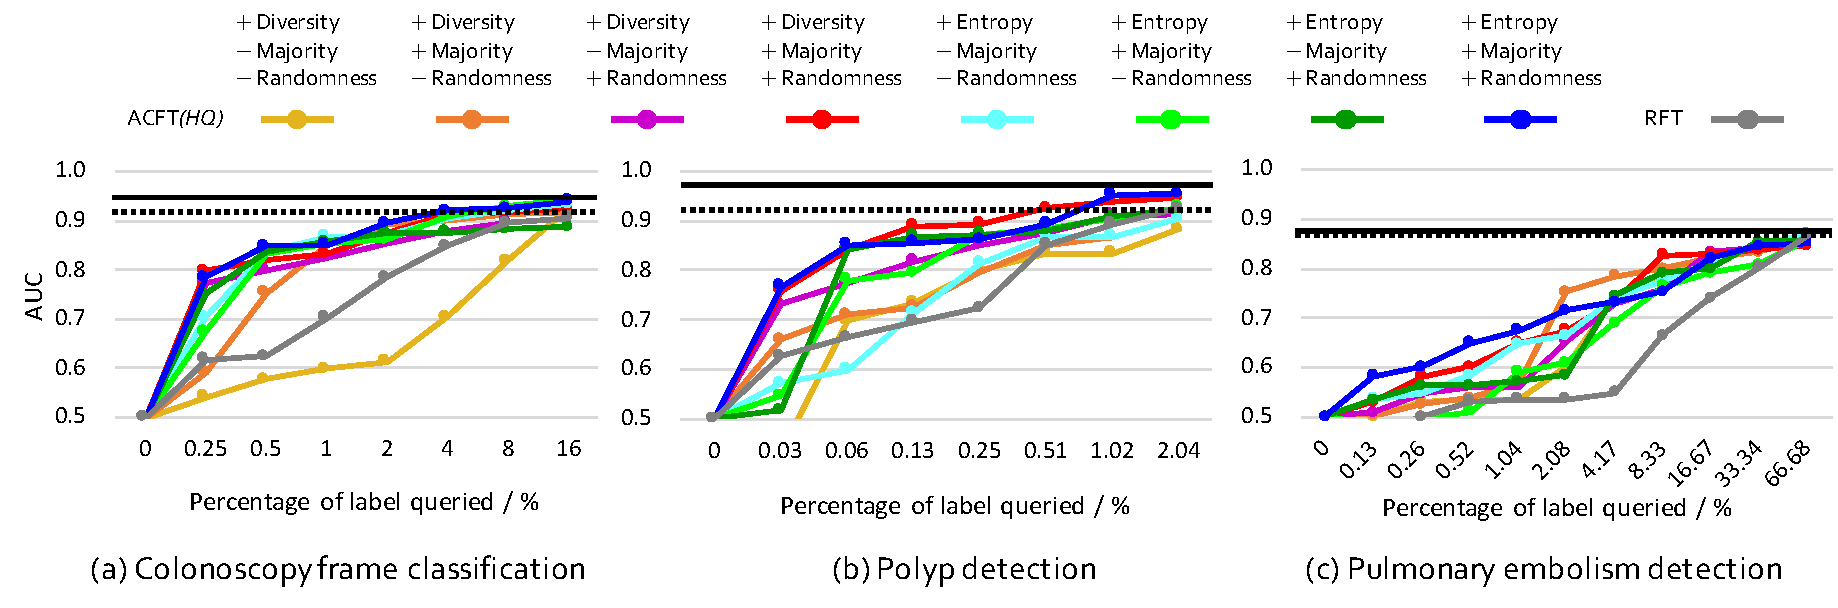
\includegraphics[width=1.0\columnwidth]{Figures/CH3/fig_selection_approaches_comparison_googlenet.pdf}
\end{center}
\caption[Assessment of Eight Active Selecting Criteria (GoogleNet)]{
Comparing eight active selection approaches with random selection on GoogLeNet~\citep{szegedy2015going} for our three distinct medical applications, including (a) colonoscopy frame classification, (b) polyp detection, and (c) pulmonary embolism detection, demonstrates consistent patterns with AlexNet. The solid black line denotes the current state-of-the-art performance of fine-tuning using full training data and the dashed black line denotes the performance of training from scratch using full training data.}
\label{ch3:fig:selection_approaches_comparison_googlenet}
\end{sidewaysfigure}

% \fillandplacepagenumber
% \end{landscape}
%%%%%%%%%%%%%%%%%%%%%%%%%%%%%%%%%%%%%%%%%%%%

%%%%%%%%%%%%%%%%%%%%%%%%%%%%%%%%%%%%%%%%%%%%
% \begin{landscape}
% \thispagestyle{empty}

% \begin{threeparttable}[t]
\begin{sidewaystable}
\scriptsize
\begin{center}
    \caption[Comparison of Learning Strategies and Selecting Criteria]{
    Comparison of proposed active learning strategies and selection criteria. As measured by the Area under the Learning Curve (ALC), bolded values in the table indicate the outstanding learning strategies (see \tableautorefname~\ref{ch3:tab:terminology}) using certain active selection criteria, and starred values represent the best performance taking both learning strategies and active selection criteria into consideration. For all three applications, we report baseline performance of random fine-tuning (RFT) using AlexNet in the table footnote. Considering the variance of random sampling for each active learning step, we conduct five independent trials for RFT and report the mean and standard deviation (mean$\pm$s.d.).}
    \label{ch3:tab:main_results}
    \begin{tabular}{p{0.1\textwidth}p{0.14\textwidth}|p{0.07\textwidth}p{0.07\textwidth}p{0.07\textwidth}p{0.07\textwidth}|p{0.07\textwidth}p{0.07\textwidth}p{0.07\textwidth}p{0.07\textwidth}}
    \hline
    Application & Learning strategy & $+$ Diversity\newline $-$ Majority\newline $-$ Random & $+$ Diversity\newline $+$ Majority\newline $-$ Random & $+$ Diversity\newline $-$ Majority\newline $+$ Random & $+$ Diversity\newline $+$ Majority\newline $+$ Random & $+$ Entropy\newline $-$ Majority\newline $-$ Random & $+$ Entropy\newline $+$ Majority\newline $-$ Random & $+$ Entropy\newline $-$ Majority\newline $+$ Random & $+$ Entropy\newline $+$ Majority\newline $+$ Random \\
    \hline
    \multirow{4}{*}{\tabincell{l}{Colonoscopy\\frame\\classification}} & ACFT$_{(Q)}$ & 0.8375 & 0.8773 & 0.8995 & 0.9160 & 0.8444 & 0.8227 & 0.9136 & 0.9061\\
    & ACFT$_{(LQ)}$ & 0.8501 & 0.8956 & 0.9083 & 0.9262 & 0.9149 & 0.9051 & 0.9033 & 0.9223\\
    & AFT$_{(LQ)}$ & \textbf{0.9183} & \textbf{0.9253} & \textbf{0.9299} & \textbf{0.9344}$^\star$ & \textbf{0.9219} & 0.9180 & \textbf{0.9268} & 0.9291\\
    & ACFT$_{(HQ)}$ & 0.9048 & 0.9236 & 0.9241 & 0.9179 & 0.9198 & \textbf{0.9266} & 0.9257 & \textbf{0.9293}\\
    \hline
    \multirow{4}{*}{\tabincell{l}{Polyp\\detection}} & ACFT$_{(Q)}$ & 0.8669 & 0.9023 & 0.8984 & 0.9168 & 0.8834 & 0.8656 & 0.9034 & 0.9271\\
    & ACFT$_{(LQ)}$ & 0.9195 & 0.9142 & \textbf{0.9497} & \textbf{0.9488} & 0.9204 & 0.9255 & \textbf{0.9475} & 0.9444\\
    & AFT$_{(LQ)}$ & \textbf{0.9242} & 0.9285 & 0.9353 & 0.9355 & 0.9292 & 0.9238 & 0.9367 & \textbf{0.9522}$^\star$ \\
    & ACFT$_{(HQ)}$ & 0.9013 & \textbf{0.9370} & 0.9116 & 0.9363 & \textbf{0.9321} & \textbf{0.9436} & 0.9196 & 0.9443\\
    \hline
    \multirow{4}{*}{\tabincell{l}{Pulmonary\\embolism\\detection}} & ACFT$_{(Q)}$ & 0.7828 & 0.7911 & 0.7690 & 0.7977 & 0.7855 & 0.7736 & 0.7296 & 0.7833\\
    & ACFT$_{(LQ)}$ & 0.8083 & \textbf{0.8176} & 0.7975 & \textbf{0.8263} & 0.8032 & \textbf{0.8086} & 0.8022 & \textbf{0.8245}\\
    & AFT$_{(LQ)}$ & 0.7650 & 0.7973 & 0.7978 & 0.8040 & 0.7917 & 0.7878 & 0.7964 & 0.8222\\
    & ACFT$_{(HQ)}$ & \textbf{0.8272}$^\star$ & 0.7876 & \textbf{0.8047} & 0.8245 & \textbf{0.8218} & 0.7995 & \textbf{0.8155} & 0.8205\\
    \hline
    \end{tabular}
    \begin{tablenotes}
        \scriptsize
        \item[1] RFT in colonoscopy frame classification: ALC = 0.8958$\pm$0.0176
        \item[2] RFT in polyp detection: ALC = 0.9358$\pm$0.0130
        \item[3] RFT in pulmonary embolism detection: ALC = 0.7849$\pm$0.0261
    \end{tablenotes}
\end{center}
\end{sidewaystable}
% \end{threeparttable}
% % }
% \fillandplacepagenumber
% \end{landscape}
%%%%%%%%%%%%%%%%%%%%%%%%%%%%%%%%%%%%%%%%%%%%

\subsection{Comparing Four Active Learning Strategies}
\label{ch3:experiment_result:comparing_four_active_learning_strategies}

As summarized in \tableautorefname~\ref{ch3:tab:terminology}, several active learning strategies can be derived. The prediction performance was evaluated according to the Area under the Learning Curve (ALC), in which the learning curve plots AUC as a function of the number of labels queried~\citep{guyon2011results}, computed on the testing dataset. \tableautorefname~\ref{ch3:tab:main_results} shows the ALC of ACFT$_{(Q)}$, ACFT$_{(LQ)}$, AFT$_{(LQ)}$ and ACFT$_{(HQ)}$ compared with RFT. Our comprehensive experiments have demonstrated that:

\begin{itemize}
    \item ACFT$_{(Q)}$ considers only newly selected candidates for fine-tuning, resulting in an unstable CNN performance due to the catastrophic forgetting of the previous samples;
    \item ACFT$_{(LQ)}$ requires a careful parameter adjustment. Although its performance is acceptable, it requires the same computing time as AFT$_{(LQ)}$, indicating that there is no advantage to continually fine-tuning the current model;
    \item AFT$_{(LQ)}$ shows the most reliable performance compared with ACFT$_{(Q)}$ and ACFT$_{(LQ)}$;
    \item The optimized version, ACFT$_{(HQ)}$, shows comparable performance to AFT$_{(LQ)}$ and occasionally outperforms AFT$_{(LQ)}$ by eliminating easy samples, focusing on hard samples, and preventing catastrophic forgetting.
\end{itemize}

In summary, our results suggest that (1) it is unnecessary to re-train models repeatedly from scratch for each active learning step and (2) learning newly annotated candidates plus a small portion of the misclassified candidates leads to equivalent performance to using the entire labeled set.


\subsection{Cutting $>$80\% Annotation Cost for Medical Applications}
\label{ch3:experiment_result:cutting_annotation_cost}


\textit{ACFT reduces 82\% annotation cost in quality assessment.} \figurename~\ref{ch3:fig:overall_result}(b) shows that ACFT, with approximately 120 candidate queries (6\%), achieves performance equivalent to a 100\% trained dataset fine-tuned from AlexNet (solid black line, AUC = 0.9366), and, with only 80 candidate queries (4\%), can achieve performance equivalent to a 100\% training dataset learned from scratch (dashed black line, AUC = 0.9204). Using only 48 candidate queries, ACFT equals the performance of RFT at 260 candidate queries. Therefore, about 81.5\% of the labeling cost associated with with RFT in colonoscopy frame classification is recovered using ACFT. Detailed analysis in \figurename~\ref{ch3:fig:selection_approaches_comparison_alexnet} and \figurename~\ref{ch3:fig:selection_approaches_comparison_googlenet} reveals that during the early stages, RFT yields performance superior to some of the active selecting processes because: 
1) random selection gives samples with the positive-negative ratio compatible with the testing and validation dataset; 2) the pre-trained model gives poor predictions in the domain of medical imaging, as it was trained by natural images. Its output probabilities are mostly inconclusive or even opposite, yielding poor selection scores. However, with randomness injected, as described in Sec.~\ref{ch3:approach_property:injecting_randomization_active_selection}, ACFT (+majority and +randomness) shows superior performance, even at early stages, with continued performance improvement during subsequent steps (see the red and blue curves in \figurename~\ref{ch3:fig:selection_approaches_comparison_alexnet} and \figurename~\ref{ch3:fig:selection_approaches_comparison_googlenet}). Besides, evidenced by \tableautorefname~\ref{ch3:tab:main_results}, ACFT performs comparably with AFT, but, unlike the latter, does not require use of the entire labeled dataset or fine-tuning from the beginning. 

\textit{ACFT reduces 86\% annotation cost in polyp detection.} \figurename~\ref{ch3:fig:overall_result}(c) shows that ACFT, with approximately 320 candidate queries (2.04\%), can achieve performance equivalent to a 100\% training dataset fine-tuned from AlexNet (solid black line, AUC = 0.9615), and, with only 10 candidate queries (0.06\%), can achieve  performance equivalent to a 100\% training dataset learned from scratch (dashed black line, AUC = 0.9358). Furthermore, ACFT, using only 20 candidate queries, achieves performance equivalent to RFT using 146 candidate queries. Therefore, nearly 86.3\% of the labeling cost associated with the use of RFT for polyp detection could be recovered with our method. The fast convergence and outstanding performance of ACFT is attributable to the majority selection and randomization method, which can both efficiently select the informative and representative candidates while excluding those with noisy labels, yet still boost the performance during the early stages. For example, the diversity criteria, if without using majority selection, would strongly favor candidates whose prediction pattern resembles Pattern C (see \tableautorefname~\ref{ch3:tab:predict_pattern}), thus performing poorer than RFT due to noisy labels generated through data augmentation.

\textit{ACFT reduces 80\% annotation cost in PE detection\footnote{I thank Jae Y. Shin, with whom I co-authored~\citet{zhou2017fine,zhou2021active}, for conducting the experiments and providing the results for PE detection.}.} \figurename~\ref{ch3:fig:overall_result}(d) shows that ACFT, with 2,560 candidate queries (66.68\%) nearly achieves performance equivalent to both the 100\% training dataset fine-tuned from AlexNet and learning from scratch (solid black line and dashed black line, where AUC = 0.8763 and AUC = 0.8706, respectively). With 320 candidate queries, ACFT can achieve the performance equivalent to RFT using 1,627 candidate queries. Based on this analysis, the cost of annotation in pulmonary embolism detection can be reduced by 80.3\% using ACFT compared with RFT.


% \subsubsection{ACFT reduces 81\% annotation cost in CIMT interpretation}
% \label{ch3:experiment_result:cutting_annotation_cost:cimt_interpretation}


\textit{ACFT reduces 35\% annotation cost in scene classification.} \figurename~\ref{ch3:fig:overall_result}(a) compares ACFT with RFT in scene classification using the \textsc{Places-3} dataset. For RFT, six different sequences are generated via systematic random sampling. The final curve is plotted showing the average performance of six runs. As shown in \figurename~\ref{ch3:fig:overall_result}(a), ACFT, with only 2,906 candidate queries, can achieve a performance equivalent to RFT with 4,452 candidate queries, as measured by the Area Under the Curve (AUC); moreover, using only 1,176 candidate queries, ACFT can achieve performance equivalent to full training using all 42,000 candidates. Therefore, 34.7\% of the RFT labeling costs and 97.2\% of full training costs could be saved using ACFT. When nearly 100\% training data are used, the performance continues to improve, suggesting that the dataset size is still insufficient, given 22 layers GoogLeNet architecture. ACFT is a general algorithm that is not only useful for medical datasets but other datasets as well, and is also effective for multi-class problems.

%%%%%%%%%%%%%%%%%%%%%%%%%%%%%%%%%%%%%%%%%%%%
% \begin{landscape}
% \thispagestyle{empty}

\begin{sidewaysfigure}
\footnotesize
\begin{center}
  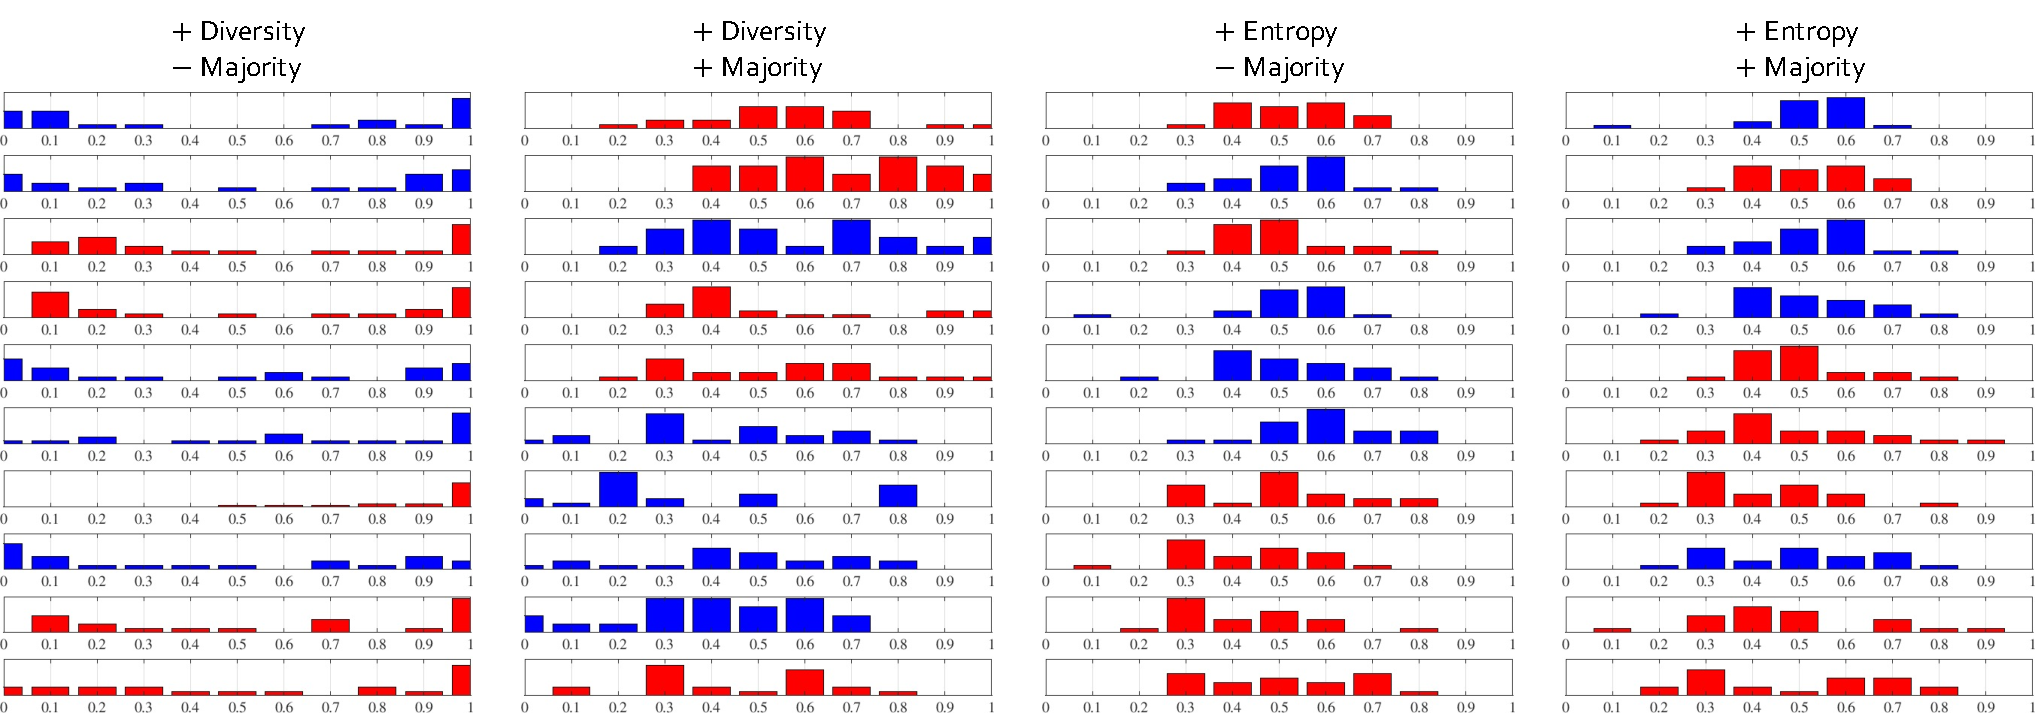
\includegraphics[width=1.0\columnwidth]{Figures/CH3/fig_predicted_distribution.pdf}
\end{center}
\caption[Prediction Distribution of Top Candidates]{
Distribution of predictions for the top ten candidates actively selected by the four ACFT methods at Step 3 in colonoscopy frame classification. Positive candidates are shown in red and negative candidates are shown in blue. This visualization confirms the assumption in \tableautorefname~\ref{ch3:tab:predict_pattern} that diversity+majority selection criteria prefers Pattern B whereas diversity suggests Pattern C; both entropy and entropy+majority favor Pattern A due to its higher degree of uncertainty. However, in this case at Step 3, with entropy+majority selection criteria, there are no more candidates with Pattern A; therefore, candidates with Pattern B are selected.
}
\label{ch3:fig:predicted_distribution}
\end{sidewaysfigure}

% \fillandplacepagenumber
% \end{landscape}
%%%%%%%%%%%%%%%%%%%%%%%%%%%%%%%%%%%%%%%%%%%%

\section{Discussion \& Conclusion}
\label{ch3:discussion_conclusion}



\subsection{What Are the Favored Prediction Patterns?}
\label{ch3:discussion_conclusion:favored_prediction_patterns}

\figurename~\ref{ch3:fig:places_examples} shows the active candidate selection process for multi-class classification. To facilitate comprehension, \tableautorefname~\ref{ch3:tab:predict_pattern} illustrates the process in the context of binary classification.
Assuming the prediction of patch $x^{j}_i$ by the current CNN is $P_i^{j}$, we call the histogram of $P_i^{j}, j \in [1, m]$ the prediction pattern of candidate $\mathcal{C}_i$. As shown in Row 1 of Table~\ref{ch3:tab:predict_pattern}, in binary classification, there are seven typical prediction patterns:
\begin{itemize}
\item Pattern A is mostly concentrated at 0.5, with a higher degree of uncertainty. Most active learning algorithms~\citep{settles2009active,guyon2011results} favor these types of candidates as they are effective for reducing uncertainty. 
\item Pattern B is flatter than Pattern A, as the patches' predictions are spread widely from 0 to 1 with a higher degree of inconsistency among the patches' predictions. Since all the patches belonging to a candidate are generated via data augmentation, they (at least the majority) are expected to make similar predictions. These types of candidates have the potential to significantly enhance the current CNN's performance.
\item Pattern C is clustered at the both ends, with a higher degree of diversity. These types of candidates are most likely associated with noisy labels at the patch level as illustrated in \figurename~\ref{ap1:fig:dataset_annotation}(c), and they are the least favorable for use in active selection because they may cause confusion when fine-tuning the CNN.
\item Patterns D and E are clustered at either end (\ie 0 or 1), with a higher degree of certainty. These types of candidates should not undergo annotation at this stage because it is likely the current CNN has correctly predicted them, and therefore these candidates would contribute very little towards fine-tuning the current CNN.
\item Patterns F and G have a higher degree of certainty for some of the patches' predictions but are associated with some outliers. These types of candidates are valuable because they are capable of smoothly improving the CNN's performance.  While such candidates might not make dramatic contributions, they do not significantly degrade the CNN's performance either.
\end{itemize}

\subsection{How Does Intra-diversity Differ from Inter-diversity?}
\label{ch3:discussion_conclusion:interdiversity_differ_from_interdiversity}

Since measuring diversity between selected samples and unlabeled samples is computationally intractable, especially for a large pool of data~\citep{sourati2016classification}, the existing diversity sampling cannot be applied directly to our real-world medical applications. To name a few, selection criteria $R$ in \citet{chakraborty2015active} involves all unlabeled samples (patches). There are 391,200 training patches for polyp detection, and computing their $R$ would demand 1.1 TB memory (391,00$^2\times$8). In addition, their algorithms for batch selection are based on the truncated power method~\citep{yuan2013truncated}, which is unable to find a solution even for our smallest application (colonoscopy frame classification with 42,000 training patches). \citet{holub2008entropy} cannot be directly used for our real-world applications either, as it has a complexity of $\mathcal{O}(L^3\times N^3)$ and requires to train $L\times N$ classifiers in each step, where $N$ indicates the number of unlabeled patches and $L$ indicates the number of classes. In addressing the computational complexity problem, we exploit the inherent consistency among the patches that are augmented from the same sample, making it feasible for our real-world applications. To contrast these two measures of diversity, the variance among samples refers to \textit{inter-diversity}, while the variance among patches augmented from the same sample refers to \textit{intra-diversity}. We recognize that intra-diversity would inevitably suffer from redundancy in selection, as it treats each sample separately and dismisses inter-diversity among samples. An obvious solution is to inject randomness into active selection criteria, as described in Sec.~\ref{ch3:approach_property:injecting_randomization_active_selection}. Nonetheless, a better solution is to combine inter- and intra-diversity together by computing inter-diversity locally on the smaller set of samples selected by intra-diversity. These solutions all aim at selecting sufficiently diverse samples with manageable computational complexity.


%%%%%%%%%%%%%%%%%%%%%%%%%%%%%%%%%%%%%%%%%%%%
\begin{figure}[t]
%\footnotesize
\begin{center}
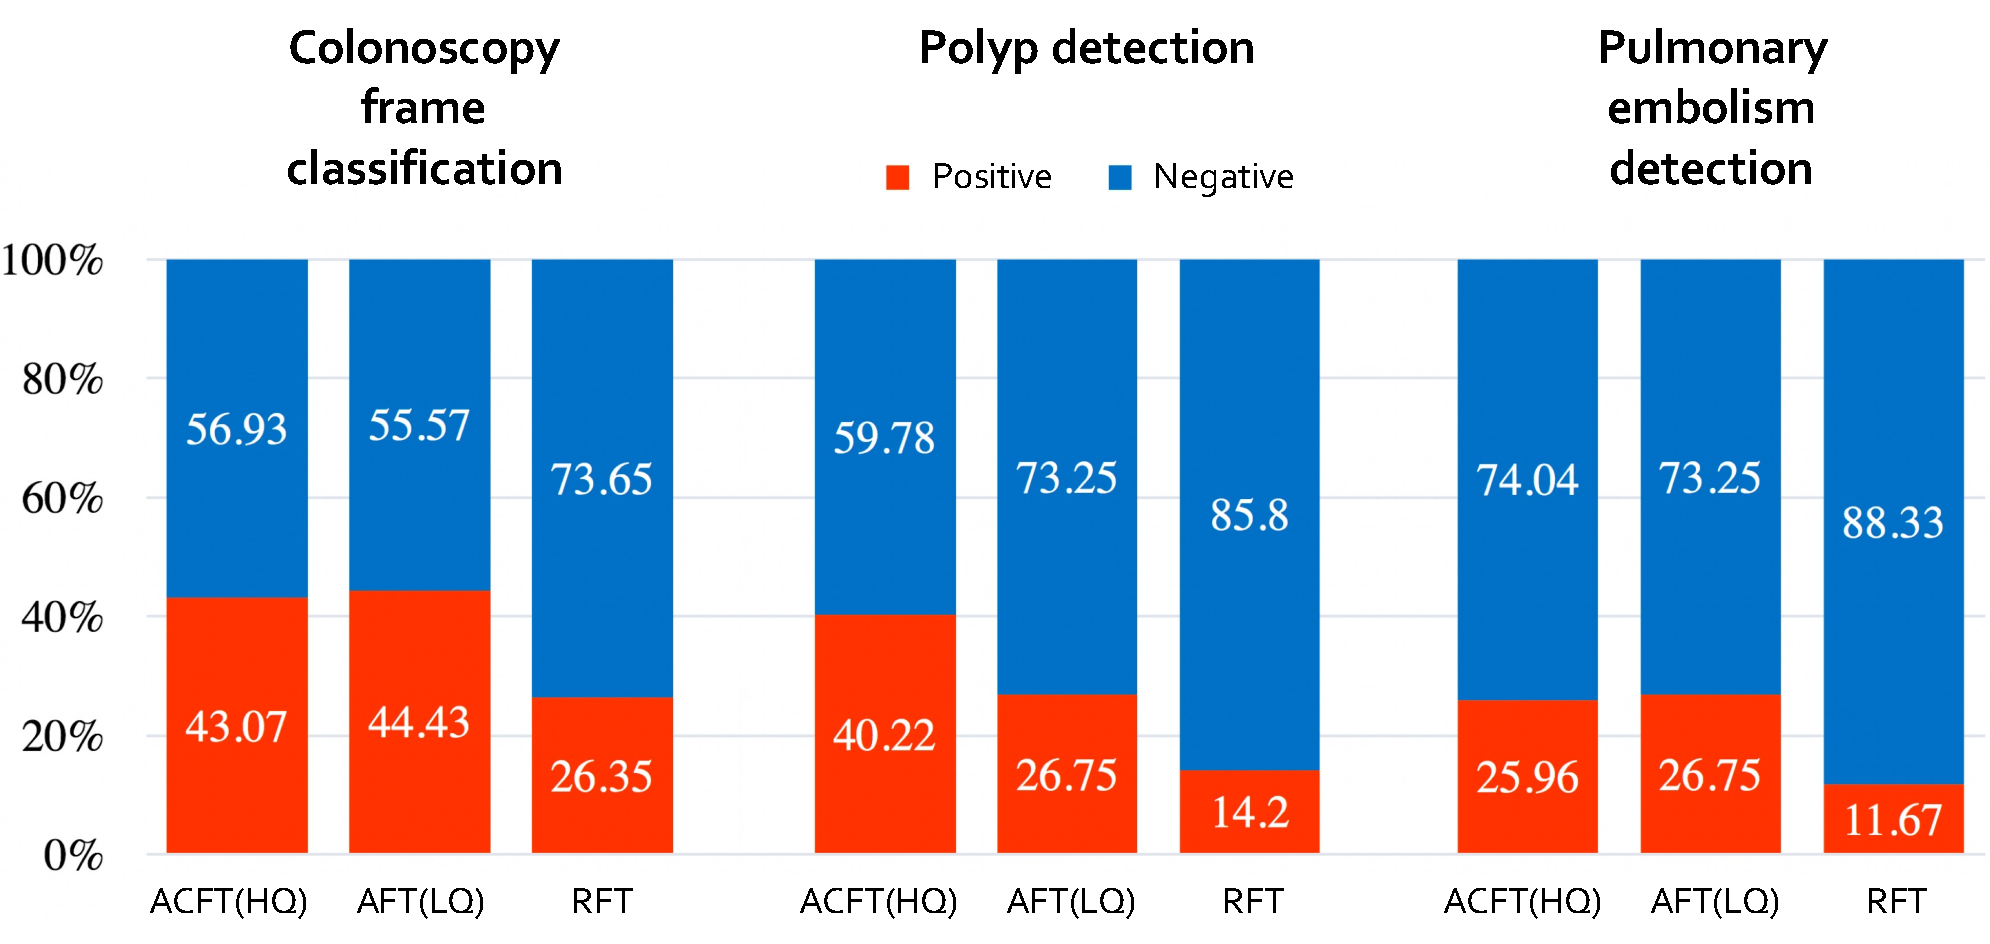
\includegraphics[width=0.9\linewidth]{Figures/CH3/fig_balance_ratio.pdf}
\end{center}
\caption[Positive/Negative Ratios of Selected Candidates]{
The positive/negative ratio in the candidates selected by ACFT, AFT and RFT. Please note that the ratio in RFT serves as an approximation for the ratio of the entire dataset.}
\label{ch3:fig:balance_ratio}
\end{figure}
%%%%%%%%%%%%%%%%%%%%%%%%%%%%%%%%%%%%%%%%%%%%

\subsection{Can Actively Selected Samples Be Automatically Balanced?}
\label{ch3:discussion_conclusion:samples_automatically_balanced}

Data is often imbalanced in real-world applications. The images of target classes of interest, \eg certain types of diseases, only appear in a small portion of the dataset. We encounter severe imbalances in our three applications. The ratio between positives and negatives is around 1:9 in the polyp and pulmonary embolism detection. Meanwhile, the ratio is approximately 3:7 in the colonoscopy frame classification. Learning from such imbalanced datasets leads to a common issue: majority bias~\citep{aggarwal2020active}, which is a prediction bias towards majority classes over minority classes. Training data should be balanced in terms of classes~\citep{japkowicz2002class,he2009learning,buda2018systematic}. Similar to most studies in active learning literature, our proposed selection criteria are not directly designed to tackle the issue of imbalance, but they have an implicit impact on balancing the data. For instance, when the current CNN has already learned more from positive samples, the next active learning selection would be more likely to prefer those negative samples, and vice-versa. On the contrary, random selection would consistently select new samples that follow roughly the same positive/negative ratio as the entire dataset. As shown in \figurename~\ref{ch3:fig:balance_ratio}, our ACFT$_{(HQ)}$ and AFT$_{(LQ)}$ are capable of automatically balancing the selected training data. After monitoring the active selection process, ACFT$_{(HQ)}$ and AFT$_{(LQ)}$ select twice as many positives compared to random selection. This does not suggest that the number of positives and negatives must be approximately identical in the selected samples. Negative samples naturally present more contextual variance than positive ones, as negatives can contain a vast array of possibilities not including the disease of interest. It is expected that the CNN should learn more from negatives to shape the decision boundary of positives. An ideal selection should cover a sufficient variety of negatives while striking an emphasis on the positives. We believe that this accounts for the quick achievement of superior performance in imbalanced data for our ACFT$_{(HQ)}$ and AFT$_{(LQ)}$.

%%%%%%%%%%%%%%%%%%%%%%%%%%%%%%%%%%%%%%%%%%%%
\begin{figure}[t]
%\footnotesize
\begin{center}
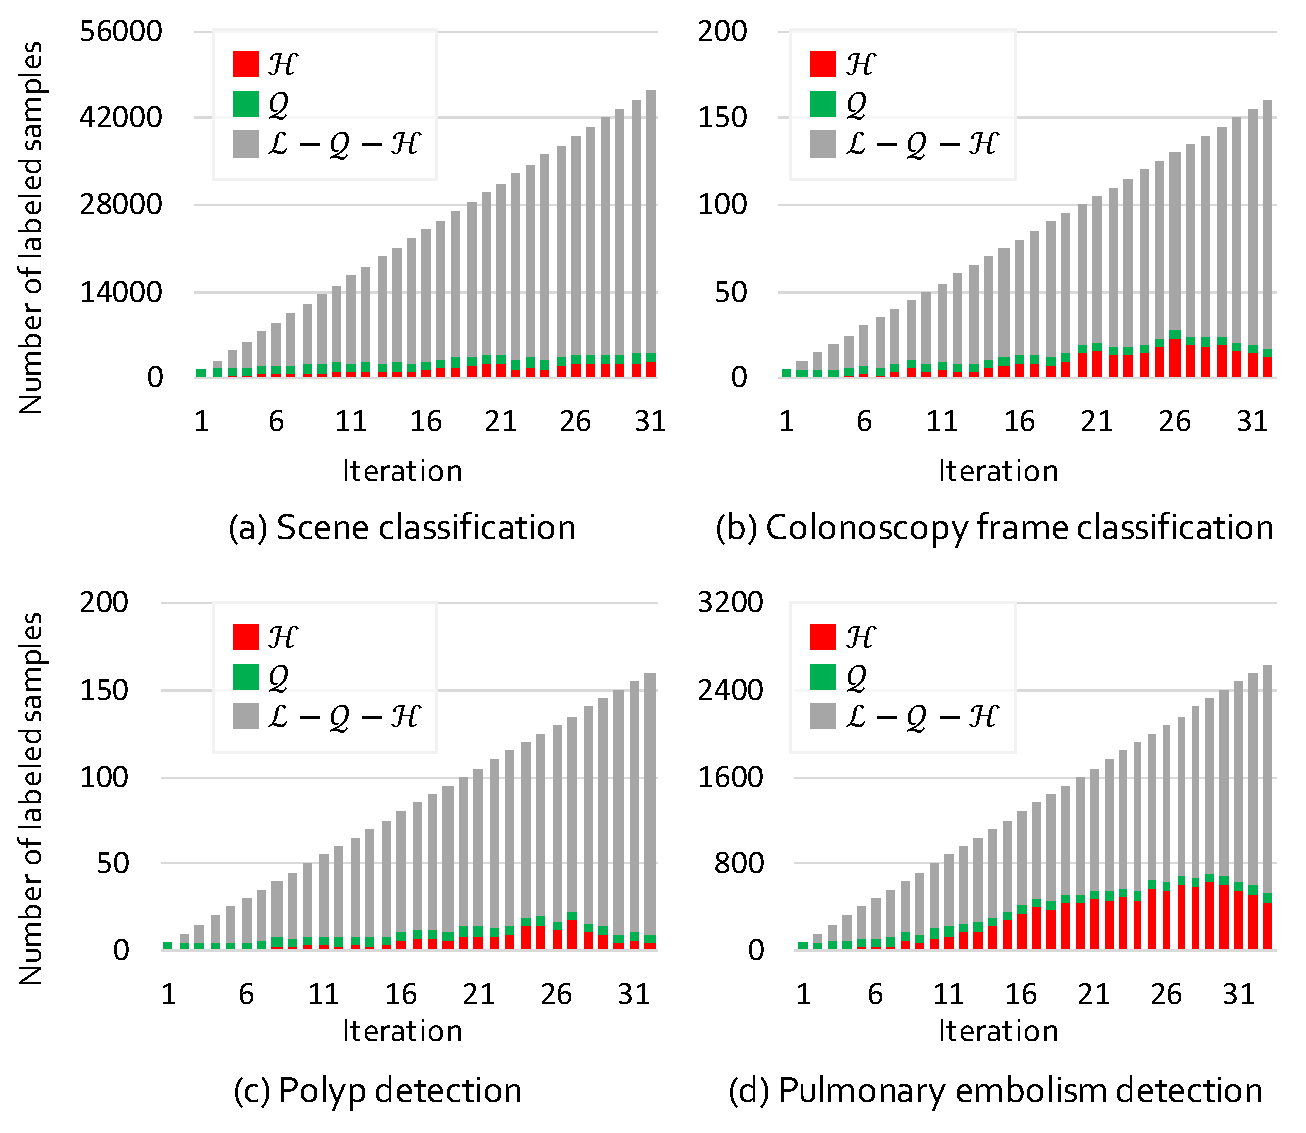
\includegraphics[width=0.75\linewidth]{Figures/CH3/fig_label_reuse.pdf}
\end{center}
\caption[Label Reusing in Active, Continual Fine-tuning]{
Labels are reused differently in four active learning strategies, as summarized in \tableautorefname~\ref{ch3:tab:terminology}. Specifically, the labels can be non-reused, partially reused, or 100\% reused. We plot the number of candidates along with each active learning step, including labeled candidates ($\mathcal{L}$), newly annotated candidates ($\mathcal{Q}$), and misclassified candidates ($\mathcal{H}$). As seen, by only continual fine-tuning on the hybrid data of $\mathcal{H}\bigcup\mathcal{Q}$, our ACFT significantly reduces training time through faster convergence than repeatedly fine-tuning on the entire labeled data of $\mathcal{L}\bigcup\mathcal{Q}$. Most importantly, as evidence by \tableautorefname~\ref{ch3:tab:main_results}, partially reusing labels can achieve compelling performance because it boosts performance by eliminating labeled easy candidates, focusing on hard ones, and preventing catastrophic forgetting.
}
\label{ch3:fig:label_reuse}
\end{figure}
%%%%%%%%%%%%%%%%%%%%%%%%%%%%%%%%%%%%%%%%%%%%

\subsection{How to Prevent Model Forgetting in Continual Learning?}
\label{ch3:discussion_conclusion:prevent_model_forgetting_continual_learning}

When a CNN learns from a stream of tasks continually, the learning of the new task can degrade the CNN's performance for earlier tasks~\citep{kirkpatrick2017overcoming,chen2018lifelong,parisi2019continual}. This phenomenon is called catastrophic forgetting, which was first recognized by~\citet{mccloskey1989catastrophic}. In our experiments, we have also observed similar behavior in active continual fine-tuning when the CNN encounters newly selected samples. This problem might not arise if the CNN is repeatedly trained on the entire labeled set at every active learning step. 
But fully reusing the labeled samples takes a lot of resources; further especially when the labeled set gets larger and larger, the impact of the newly selected samples on the model training becomes smaller and smaller (relative to the whole labeled set).
To make the training more efficient and maximize the contribution of new data, we attempted to fine-tune the CNN only on the newly selected samples, developing the learning strategy called ACFT$_{(Q)}$. However, as seen in~\tableautorefname~\ref{ch3:tab:main_results}, ACFT$_{(Q)}$ results in a substantially unstable performance because of the catastrophic forgetting. To track the forgotten samples, we have plotted a histogram of the misclassified candidates ($\mathcal{H}$) by the current CNN against labeled candidates ($\mathcal{L}$) and newly selected candidates ($\mathcal{Q}$) in~\figurename~\ref{ch3:fig:label_reuse}. We found that if the CNN is only fine-tuned on the newly selected samples at each step, it tends to forget the samples that have been learned from previous steps. This is because new data will likely override the weights that have been learned in the past, and thus overfitting the CNN on this data and degrading the model's generalizability. Therefore, we propose to combine the newly selected ($\mathcal{Q}$) and misclassified ($\mathcal{H}$) candidates together to continual fine-tune the current CNN, which not only spotlights the power of new data to achieve the comparable performance (see~\tableautorefname~\ref{ch3:tab:main_results}: ACFT$_{(HQ)}$ vs. AFT$_{(LQ)}$), but also eases the computational cost by eliminating re-training on easy samples, focusing on hard ones, and preventing catastrophic forgetting. 

\subsection{Is ACFT Generalizable to Other Models?}
\label{ch3:discussion_conclusion:generalizable_other_models}

We based our experiments on AlexNet and GoogLeNet. Alternatively, deeper architectures, such as VGG~\citep{simonyan2014very}, ResNet~\citep{he2016deep}, DenseNet~\citep{huang2017densely}, and FixEfficientNet~\citep{touvron2020fixing}, could have been used and they are known to show relatively higher performance for challenging computer vision tasks.
However, the purpose of this work is not to achieve the highest performance for different medical image tasks but to answer a critical question: {\em How can annotation costs be significantly reduced when applying CNNs to medical imaging?} For this purpose, we have experimented with our three applications, demonstrating consistent patterns between AlexNet and GoogLeNet as shown in \figurename~\ref{ch3:fig:selection_approaches_comparison_alexnet} and \figurename~\ref{ch3:fig:selection_approaches_comparison_googlenet}. As a result, given this generalizability, we can focus on comparing the prediction patterns and learning strategies rather than running experiments on different CNN architectures. Moreover, our active selection criteria only rely on data augmentation and model prediction, without being tied to specific types of predictors. This suggests that not only various CNN architectures, but also other predictive methods---spanning old fashions (\eg SVM, Random Forests, and AdaBoost) to recent trends such as CapsuleNet~\citep{sabour2017dynamic} and Transformer~\citep{dosovitskiy2020image}---can benefit from the progress in active learning.

\subsection{Can We Do Better on the Cold Start Problem?}
\label{ch3:discussion_conclusion:cold_start_problem}

It is crucial to intelligently select initial samples for an active learning procedure, especially for algorithms like our ACFT, which starts from a completely empty labeled dataset. Our results in \figurename~\ref{ch3:fig:selection_approaches_comparison_alexnet} and \figurename~\ref{ch3:fig:selection_approaches_comparison_googlenet} and several other studies~\citep{borisov2010active,zhou2017fine,yuan2020cold,gao2020consistency} reveal that uniformly, randomly selecting initial samples from the unlabeled set could outperform active selection at the beginning. This is one of the most challenging problems in active learning, known as the \textit{cold start} problem, which is ascribed to (1) data scarcity and (2) model instability at early stages. 
First, the data distribution in randomly selected samples better reflects the original distribution of the entire dataset than in actively selected samples. Maintaining a similar distribution between training and test data is beneficial when using scarce data. The most common practice is to admit the power of randomness at the beginning and randomly select initial samples from the unlabeled set~\citep{ren2020survey}. Our ACFT addresses the cold start problem by incorporating a random sampling probability with respect to the active selection criteria (as detailed in Sec.~\ref{ch3:approach_property:injecting_randomization_active_selection}). The devised ACFT (+randomness vs. -randomness in \figurename~\ref{ch3:fig:selection_approaches_comparison_alexnet} and \figurename~\ref{ch3:fig:selection_approaches_comparison_googlenet}) shows superior performance, even in early stages, with continued performance improving during the subsequent steps. 
Second, in the beginning, the CNN understandably fails to amply predict new samples, as it is trained with an inadequate number of samples. With horrible predictions, no matter how marvelous the selection criterion is, the selected samples would be unsatisfactory---as said ``garbage in garbage out''. To express meaningful CNN predictions, our ACFT suggests the use of pre-trained CNNs (as illustrated in Alg.~\ref{ch3:alg:ACFT}), not only initializing the CNN at the first step, but also providing fairly reasonable predictions for initial active selection. \figurename~\ref{ch3:fig:overall_result} presents encouraging results of active selection using pre-trained CNNs compared with random sampling from the unlabeled set (ACFT vs. RFT).
However, a CNN pre-trained on \textsc{ImageNet} may give poor predictions in the medical imaging domain, as it was trained from only {\em natural} images; it is associated with a large domain gap for medical images. As a result, the CNN predictions may be inconclusive or even opposite, yielding poor selection scores. Naturally, one may consider utilizing pre-trained models in the same domains to reduce this domain gap~\citep{zhou2021models,haghighi2020learning,feng2020parts2whole}. \citet{yuan2020cold} has demonstrated this idea in natural language processing by applying self-supervised language modeling to select initial samples. In the case of medical imaging, we naturally expect that self-supervised methods can also mitigate the pronounced domain gap between natural and medical imaging, offering a great starting point for selecting samples using domain-relevant image representation. More importantly, the learning objectives in self-supervised methods are applicable for discovering the most representative initial samples. 
For instance, our diversity criterion shares a similar spirit with the learning objective of BYOL~\citep{grill2020bootstrap} and of Parts2Whole~\citep{feng2020parts2whole}, as they all aim to pull together the patches augmented from the same sample.
Therefore, their objective functions could serve as an off-the-shelf measure for the power of a sample in elevating the pre-trained CNN's performance. The underlying hypothesis is that the worthiness of labeling a sample correlates with the learning objective of self-supervised pre-training. Specifically, a sample is potentially more worthy to train the CNN if it requires considerably more effort to perform the task of in-painting~\citep{pathak2016context}, restoration~\citep{zhou2021models}, contrastive learning~\citep{chen2020simple}, or colorization~\citep{zhang2016colorful}. We anticipate that self-supervised methods have great potential to accommodate the selection of initial samples by leveraging unlabeled data in the same domain, therefore, more effectively addressing the cold start problem in active learning. 

\subsection{Is Our Consistency Observation Useful for Other Purposes?}
\label{ch3:discussion_conclusion:consistency_observation_other_purposes}

Our key observation is that all patches augmented from the same sample share the same label, and thus are expected to have similar predictions by the CNN. This inherent invariance allows us to devise the diversity metric for estimating the worthiness of labeling the sample. From a broader view, the use of data consistency before and after a mixture of augmentation has played an important role in many other circumstances. In semi-supervised learning, the consistency loss serves as a bridge between labeled and unlabeled data. While the CNN is trained on labeled data, the consistency loss constrains predictions to be invariant to unlabeled data augmented in varying ways~\citep{yu2019uncertainty,cui2019semi,bortsova2019semi,fotedar2020extreme,gao2020consistency}. In self-supervised learning, the concept of consistency allows CNNs to learn transformation invariance features by either always restoring the original image from the transformed one~\citep{zhu2020rubik,zhou2021models} or explicitly pulling all patches augmented from the same image together in the feature space~\citep{feng2020parts2whole,chen2020simple,he2020momentum}. Albeit the great promises of consistency loss, automatic data augmentation inevitably generates ``noisy'' samples, jeopardizing the data consistency presumption. As an example, when an image contains objects A and B, random cropping may miss either one of the objects fully or partially, causing label inconsistency or representation inconsistency~\citep{purushwalkam2020demystifying,hinton2021represent}. Therefore, the choice of data augmentation is critical in employing the data consistency presumption. Other than data consistency, the prediction consistency of model ensembles can also calculate the diversity. For instance, \citet{gal2016dropout,gal2017deep,tsymbalov2018dropout} have proposed to estimate the prediction diversity presented in the CNN via Monte-Carlo dropout in the inference;~\citet{beluch2018power,yang2017suggestive,kuo2018cost,li2020transformation,venturini2020uncertainty} measure the prediction consistency by feeding images to multiple independent CNNs that have been trained for the same data and purpose. Unlike the data consistency in our work, their presumption is the model consistency, wherein the CNN predictions ought to be consistent if the same sample goes through the model ensembles; otherwise, this sample is considered worthy of labeling.


\subsection{Conclusion and Broader Impacts}
\label{ch3:discussion_conclusion:conclusion_broader_impacts}

We have developed a novel method for dramatically reducing annotation cost by integrating active learning and transfer learning. Compared with the state-of-the-art random selection method~\citep{tajbakhsh2016convolutional}, our method can reduce the annotation cost by at least half for three medical applications and by more than 33\% for natural image dataset \textsc{Places-3}. The superior performance of our method is attributable to eight distinct advantages, detailed in Sec.~\ref{ch3:approach_property:several_unique_properties}. We believe that labeling at the candidate level offers a sensible balance for our three applications, whereas labeling at the patient level would certainly enhance annotation cost reduction, but introduces more severe label noise. Labeling at the patch level compensates for additional label noise but would impose significant burdens on experts for annotation creation. More importantly, our method has the potential to positively impact computer-aided diagnosis (CAD) in medical imaging. The current regulations require that CAD systems be deployed in a ``closed'' environment, in which all CAD results are reviewed and errors, if any, must be corrected by radiologists. As a result, all false positives are dismissed and all false negatives are supplied, an instant on-line feedback process that makes it possible for CAD systems to be self-learning and self-improving after deployment given the continual fine-tuning capability of our method.

We presented this work in our CVPR paper~\citep{zhou2017fine} to integrate active learning and deep learning via continual fine-tuning. It has since been quickly adopted by the research community: reviewed by some of the most prestigious journals and conferences in the field~\citep{wang2018uncertainty,zhang2019attention,sourati2019intelligent,liu2019exploiting,bi2019active,zhang2019medical,budd2019survey}, served as competitive baseline~\citep{shi2019active,duan2019improved}, and enlightened to develop more advanced active learning approaches~\citep{zhou2019integrating,li2019reverse,zhang2019using}. Moreover, although the technique was derived from the medical context, it is a general active learning approach, which has been adopted in multiple alternative fields such as text classification~\citep{oftedal2019uncertainty}, vehicle type recognition~\citep{huang2019cost}, streaming recommendation system~\citep{guo2019streaming}, etc.



% \section*{Acknowledgements}

% I thank R. Todd Hurst for allowing us to test our ideas on the CIMT dataset.